\documentclass{article}
\usepackage[final]{nips_2017}
\usepackage{polski}
\usepackage[utf8]{inputenc}    % allow utf-8 input
\usepackage[T1]{fontenc}       % use 8-bit T1 fonts
\usepackage{hyperref}          % hyperlinks
\usepackage{url}               % simple URL typesetting
\usepackage{booktabs}          % professional-quality tables
\usepackage{amsfonts}          % blackboard math symbols
\usepackage{nicefrac}          % compact symbols for 1/2, etc.
\usepackage{microtype}         % microtypography
\usepackage[section]{placeins} % figures kept in sections
\usepackage{graphicx}          % images
\graphicspath{ {./img/} }
\usepackage{multirow}
\usepackage{float}             % figures in place
\usepackage{caption}		   % smaller margin after figure

\renewcommand{\figurename}{Wykres}
\setlength{\belowcaptionskip}{-20pt}

\title{  Sieć konwolucyjna\\Sieci Neuronowe 2020 }

\author{
  Jakub Ciszek \\
  238035\\
}

\begin{document}

\maketitle

\newpage
\tableofcontents
\newpage

Cały kod wykorzystany w zadaniu znajduje się pod adresem: \url{https://github.com/Greenpp/sieci-neuronowe-pwr-2020}

\section{Opis badań}
\subsection{Plan eksperymentów}

Wszystkie eksperymenty zostały przeprowadzone 10 razy. Losowość przy inicjalizacji wag oraz generacji danych nie została narzucona żadnym ziarnem. Podczas badań przyjęto górną granicę 10 epok, po przekroczeniu której, uczenie zostawało przerywane. Ze względu na charakter zadania (klasyfikacja) na ostatniej warstwie użyto funkcji Softmax, a za funkcję straty przyjęto Entropię krzyżową. Użyta sieć składała się z warstwy konwolucyjnej, max pool, oraz w pełni połączonej ze 128 neuronami. Wagi były inicjalizowane metodą He, a uczenie przebiegało przy pomocy metody Adam. Jako funkcję aktywacji przyjęto ReLU.
Z powodów wydajnościowych testowanie modelu przeprowadzano co każde 32 paczki, z których każda składała się z 32 przykładów.\\
Zgodnie z instrukcją zostały przeprowadzone następujące badania:
\begin{itemize}
	\item Wpływ wielkości filtra na przebieg procesu uczenia
	\item Porównanie z MLP    
\end{itemize}
Podczas wizualizacji funkcji straty pominięto pierwsze 10 pomiarów dla lepszej czytelności.

\subsection{Charakterystyka zbiorów danych}

Danymi użytymi w zadaniu jest zbiór ręcznie pisanych cyfr \(0-9\) - MNIST. Na zbiór składa się 70,000 obrazów wielkości 28x28 pikseli. Na wyjściu znajduje się 10 klasom na wyjściu. Użyta w zadaniu wersja została podzielona na 3 zbiory:
\begin{itemize}
	\item Uczący - 50,000 przykładów.
	\item Walidujący - 10,000 przykładów.
	\item Testowy - 10,000 przykładów.
\end{itemize}
W trakcie eksperymentów wykorzystano jedynie zbiory uczący i testowy.

\newpage
\section{Eksperymenty}

\subsection{Wpływ wielkości filtra na przebieg procesu uczenia}
\subsubsection*{Założenia}

Zmienną w tym eksperymencie była wielkość filtra, przyjmowała wartości ze zbioru \(\{$2, 3, 4, 5$\}\)
\subsubsection*{Przebieg}

Podczas eksperymentu model został zainicjalizowany 10 razy dla każdej z badanych wartości oraz wyuczony, uzyskane wyniki zostały zapisane w postaci pliku .plk do dalszej analizy.

\subsubsection*{Wyniki}
\begin{figure}[H]
	\centering
	\caption{Dokładność modelu w zależności od wielkości filtra}
	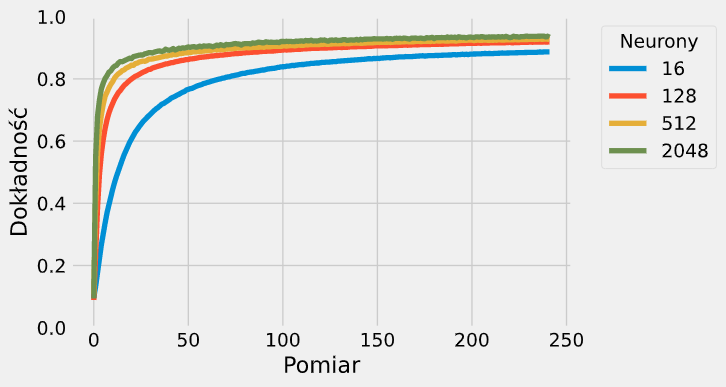
\includegraphics[width=\textwidth]{hidden_acc.png}
	\label{fig:res11}
\end{figure}

\begin{table}[H]
	\caption{Średnia maksymalna dokładność w zależności od wielkości filtra}
	\label{tabela-res-11}
	\centering
	\begin{tabular}{rrr}
		\toprule
		Wielkość filtra & Dokładność [\%] \\
		\midrule
		2                 & --                 \\
		3                 & --                 \\
		4                 & --                 \\
		5                 & --                 \\
		\bottomrule
	\end{tabular}
\end{table}

\subsubsection*{Wnioski}

TODO

\newpage
\subsection{Porównanie z MLP}
\subsubsection*{Założenia}
\begin{table}[H]
	\caption{Stałe dla eksperymentu 2}
	\label{tabela-const-2}
	\centering
	\begin{tabular}{lr}
		\toprule
		Parametr          & Wartość \\
		\midrule
		Wielkość filtra & --        \\
		\bottomrule
	\end{tabular}
\end{table}

\subsubsection*{Przebieg}

Podczas eksperymentu model został zainicjalizowany 10 razy dla każdej z badanych wartości oraz wyuczony, uzyskane wyniki zostały zapisane w postaci pliku .plk do dalszej analizy.

\subsubsection*{Wyniki}
\begin{figure}[H]
	\centering
	\caption{Porównanie dokładności modeli}
	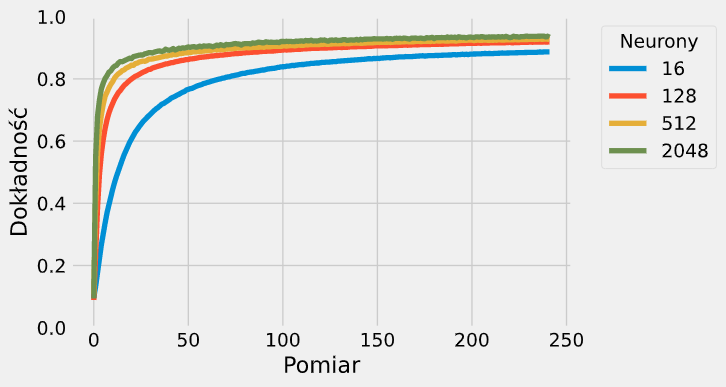
\includegraphics[width=\textwidth]{hidden_acc.png}
	\label{fig:res21}
\end{figure}

\begin{table}[H]
	\caption{Średnia maksymalna dokładność w zależności od modelu}
	\label{tabela-res-21}
	\centering
	\begin{tabular}{rrr}
		\toprule
		Przykłady & Dokładność [\%] \\
		\midrule
		MLP        & --                 \\
		Konwolucja & --                 \\
		\bottomrule
	\end{tabular}
\end{table}

\subsubsection*{Wnioski}

TODO

\newpage
\section{Wnioski}

\begin{itemize}
	\item TODO
\end{itemize}

\end{document}